%----------------------------------------------------------------
%
%  File    :  vpn_evaluation.tex
%
%  Author  :  Keith Andrews, IICM, TU Graz, Austria
% 
%  Created :  22 Feb 96
% 
%  Changed :  19 Feb 2004
% 
%----------------------------------------------------------------

\chapter{Evaluation}

\label{chap:Evaluation}
test
\section{Learning Results} \label{subsec:learnresults}
% section where we show and analyze reference and no filter models including model and statistics
TODO: show and analyze Reference and NoFilter model versions --> Maybe move them here from previous chapter?

\begin{figure}[h]
	\centering
	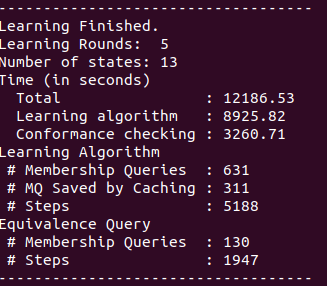
\includegraphics[width=0.7\linewidth]{images/NoFilterA}
	\caption{Most common learned model.}
	\label{fig:nofiltera}
\end{figure}

\begin{figure}[h]
	\centering
	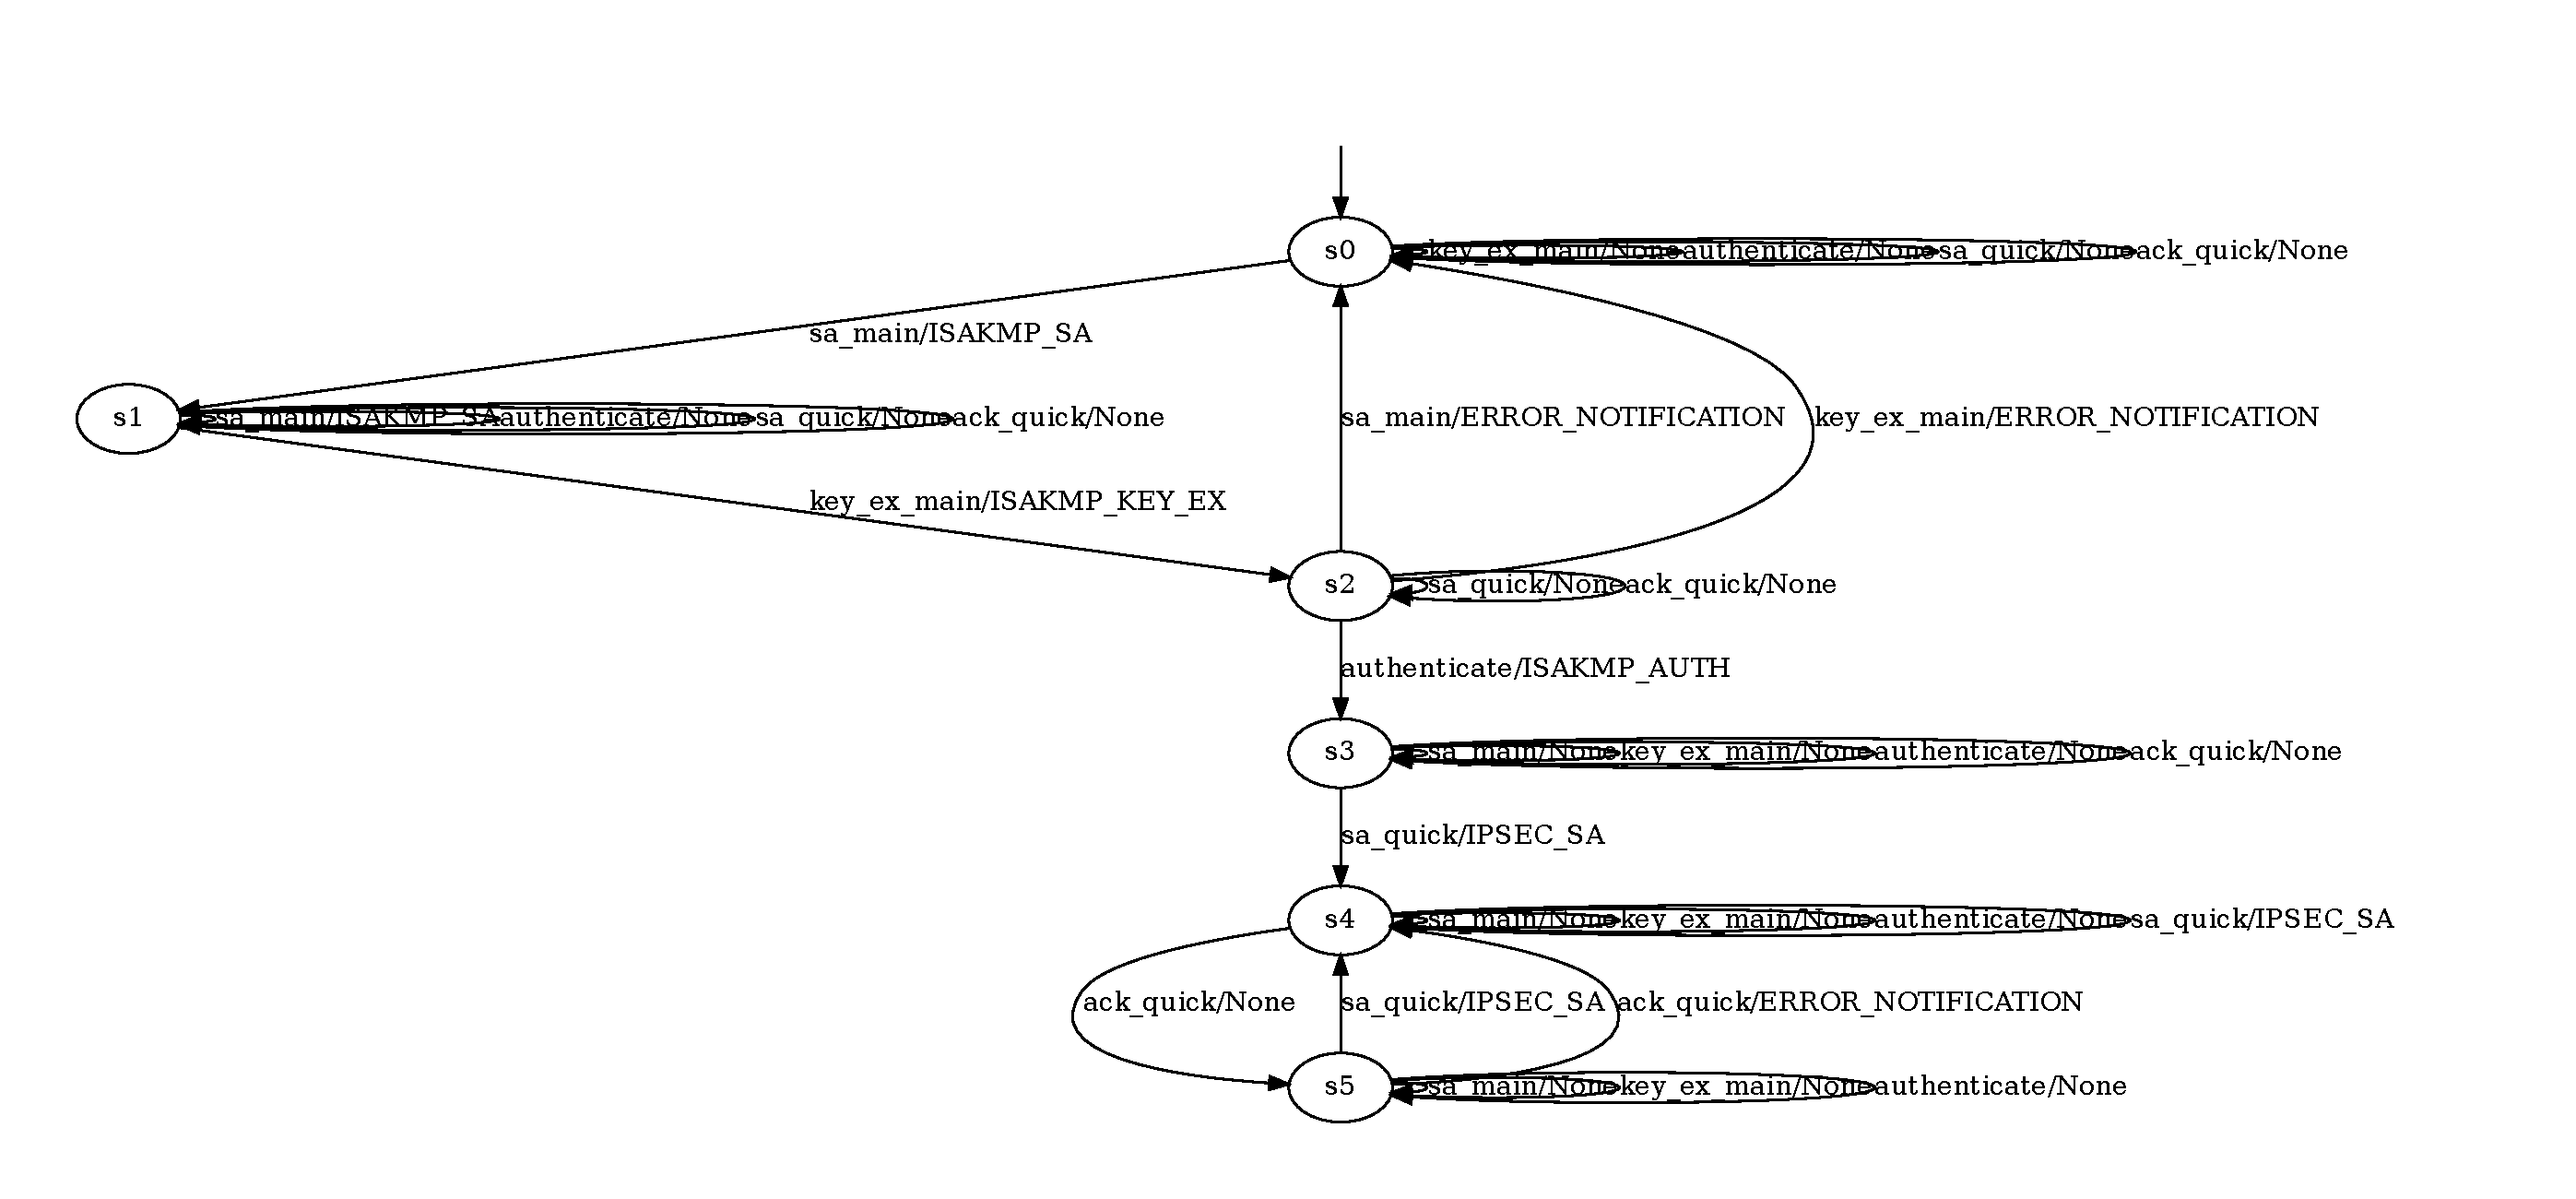
\includegraphics[width=0.9\linewidth]{images/Reference}
	\caption{Clean model learned using retransmission filtering}
	\label{fig:reference}
\end{figure}


% Error model
TODO: analyze error model

\begin{figure}
	\centering
	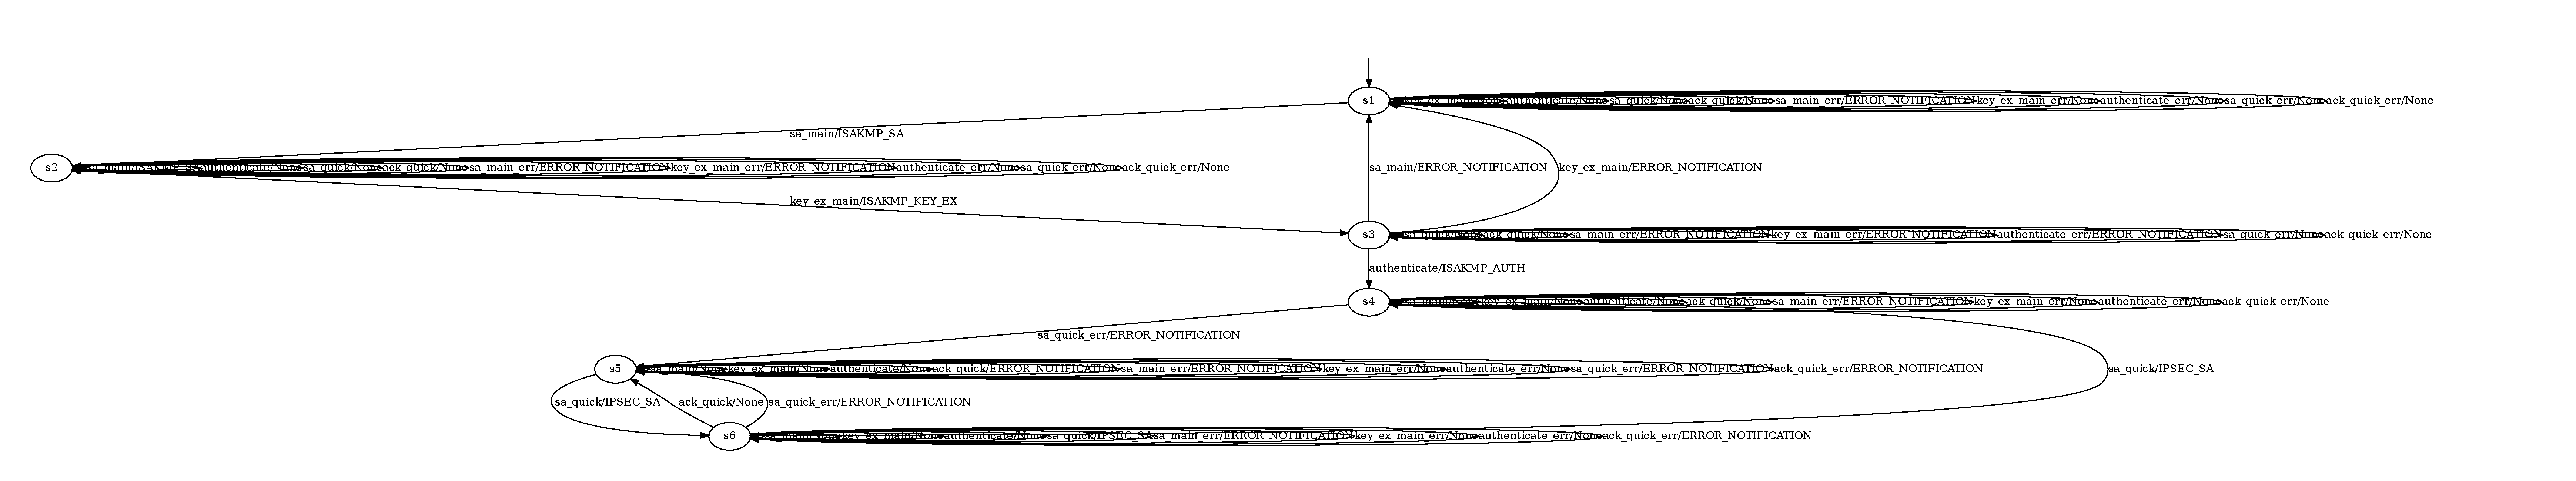
\includegraphics[width=\linewidth]{images/WithFilterWithErrors}
	\caption{Model with malformed messages}
	\label{fig:withfilterwitherrors}
\end{figure}


% section copmaring KV and Lstar
TODO: Compare KV and Lstar

% section with discovered bug
TODO: Expand on this
faulty library fixes --> a persistent bug that even after several weeks of debugging. Initially we believed this to be caused by non-deterministic behavior of the SUL or problems in our code, but after comparing logs and packet captures, still occasionally would exhibit non-deterministic behavior and therefore crash. Bug appeared to occur randomly at different points during the learning process. Additionally, it did not occur consistently each learning attempt, which made debugging even more difficult. Finally we discovered a very niche bug in a used Diffie-Hellman python library where if the most significant byte was a zero, it would be omitted from the response, causing the local result to be different than the values calculated by the server. As this would only occur in the rare case where the MSB of the DH exchange was zero, this explains the random and difficult to reproduce behavior of the bug. As the library is not a very widespread one, the impact of this bug is presumably not all that high, still it might compromise the security of affected systems and the maintainer has been notified of the problem.

No way this bug would have been found with out the exhaustive testing done by the model learning procedure and without seeing the slight differences in the resulting models that did not crash during the learning process.
\section{Fuzzing Results} \label{subsec:fuzzresults}
test
% Two main parts, eval of learning and eval of testing